\documentclass[11pt,a4paper,]{article}
\usepackage{lmodern}

\usepackage{amssymb,amsmath}
\usepackage{ifxetex,ifluatex}
\usepackage{fixltx2e} % provides \textsubscript
\ifnum 0\ifxetex 1\fi\ifluatex 1\fi=0 % if pdftex
  \usepackage[T1]{fontenc}
  \usepackage[utf8]{inputenc}
\else % if luatex or xelatex
  \usepackage{unicode-math}
  \defaultfontfeatures{Ligatures=TeX,Scale=MatchLowercase}
\fi
% use upquote if available, for straight quotes in verbatim environments
\IfFileExists{upquote.sty}{\usepackage{upquote}}{}
% use microtype if available
\IfFileExists{microtype.sty}{%
\usepackage[]{microtype}
\UseMicrotypeSet[protrusion]{basicmath} % disable protrusion for tt fonts
}{}
\PassOptionsToPackage{hyphens}{url} % url is loaded by hyperref
\usepackage[unicode=true]{hyperref}
\hypersetup{
            pdftitle={FFORMS: Feature-based FORecast Model Selection},
            pdfkeywords={Algorithm selection problem, Time series, Random forest, Machine learning interpretability},
            pdfborder={0 0 0},
            breaklinks=true}
\urlstyle{same}  % don't use monospace font for urls
\usepackage{geometry}
\geometry{left=2.5cm,right=2.5cm,top=2.5cm,bottom=2.5cm}
\usepackage[style=authoryear-comp,]{biblatex}
\addbibresource{references.bib}
\usepackage{longtable,booktabs}
% Fix footnotes in tables (requires footnote package)
\IfFileExists{footnote.sty}{\usepackage{footnote}\makesavenoteenv{long table}}{}
\IfFileExists{parskip.sty}{%
\usepackage{parskip}
}{% else
\setlength{\parindent}{0pt}
\setlength{\parskip}{6pt plus 2pt minus 1pt}
}
\setlength{\emergencystretch}{3em}  % prevent overfull lines
\providecommand{\tightlist}{%
  \setlength{\itemsep}{0pt}\setlength{\parskip}{0pt}}
\setcounter{secnumdepth}{5}

% set default figure placement to htbp
\makeatletter
\def\fps@figure{htbp}
\makeatother


\title{FFORMS: Feature-based FORecast Model Selection}

%% MONASH STUFF

%% CAPTIONS
\RequirePackage{caption}
\DeclareCaptionStyle{italic}[justification=centering]
 {labelfont={bf},textfont={it},labelsep=colon}
\captionsetup[figure]{style=italic,format=hang,singlelinecheck=true}
\captionsetup[table]{style=italic,format=hang,singlelinecheck=true}

%% FONT
\RequirePackage{bera}
\RequirePackage{mathpazo}

%% HEADERS AND FOOTERS
\RequirePackage{fancyhdr}
\pagestyle{fancy}
\rfoot{\Large\sffamily\raisebox{-0.1cm}{\textbf{\thepage}}}
\makeatletter
\lhead{\textsf{\expandafter{\@title}}}
\makeatother
\rhead{}
\cfoot{}
\setlength{\headheight}{15pt}
\renewcommand{\headrulewidth}{0.4pt}
\renewcommand{\footrulewidth}{0.4pt}
\fancypagestyle{plain}{%
\fancyhf{} % clear all header and footer fields
\fancyfoot[C]{\sffamily\thepage} % except the center
\renewcommand{\headrulewidth}{0pt}
\renewcommand{\footrulewidth}{0pt}}

%% MATHS
\RequirePackage{bm,amsmath}
\allowdisplaybreaks

%% GRAPHICS
\RequirePackage{graphicx}
\setcounter{topnumber}{2}
\setcounter{bottomnumber}{2}
\setcounter{totalnumber}{4}
\renewcommand{\topfraction}{0.85}
\renewcommand{\bottomfraction}{0.85}
\renewcommand{\textfraction}{0.15}
\renewcommand{\floatpagefraction}{0.8}

%\RequirePackage[section]{placeins}

%% SECTION TITLES
\RequirePackage[compact,sf,bf]{titlesec}
\titleformat{\section}[block]
  {\fontsize{15}{17}\bfseries\sffamily}
  {\thesection}
  {0.4em}{}
\titleformat{\subsection}[block]
  {\fontsize{12}{14}\bfseries\sffamily}
  {\thesubsection}
  {0.4em}{}
\titlespacing{\section}{0pt}{*5}{*1}
\titlespacing{\subsection}{0pt}{*2}{*0.2}


%% TITLE PAGE
\def\Date{\number\day}
\def\Month{\ifcase\month\or
 January\or February\or March\or April\or May\or June\or
 July\or August\or September\or October\or November\or December\fi}
\def\Year{\number\year}

\makeatletter
\def\wp#1{\gdef\@wp{#1}}\def\@wp{??/??}
\def\jel#1{\gdef\@jel{#1}}\def\@jel{??}
\def\showjel{{\large\textsf{\textbf{JEL classification:}}~\@jel}}
\def\nojel{\def\showjel{}}
\def\addresses#1{\gdef\@addresses{#1}}\def\@addresses{??}
\def\cover{{\sffamily\setcounter{page}{0}
        \thispagestyle{empty}
        \placefig{2}{1.5}{width=5cm}{monash2}
        \placefig{16.9}{1.5}{width=2.1cm}{MBusSchool}
        \begin{textblock}{4}(16.9,4)ISSN 1440-771X\end{textblock}
        \begin{textblock}{7}(12.7,27.9)\hfill
        
\includegraphics[height=0.7cm]{AACSB}~~~
        
\includegraphics[height=0.7cm]{EQUIS}~~~
        
\includegraphics[height=0.7cm]{AMBA}
        \end{textblock}
        \vspace*{2cm}
        \begin{center}\Large
        Department of Econometrics and Business Statistics\\[.5cm]
        \footnotesize http://monash.edu/business/ebs/research/publications
        \end{center}\vspace{2cm}
        \begin{center}
        \fbox{\parbox{14cm}{\begin{onehalfspace}\centering\Huge\vspace*{0.3cm}
                \textsf{\textbf{\expandafter{\@title}}}\vspace{1cm}\par
                \LARGE\@author\end{onehalfspace}
        }}
        \end{center}
        \vfill
                \begin{center}\Large
                \Month~\Year\\[1cm]
                Working Paper \@wp
        \end{center}\vspace*{2cm}}}
\def\pageone{{\sffamily\setstretch{1}%
        \thispagestyle{empty}%
        \vbox to \textheight{%
        \raggedright\baselineskip=1.2cm
     {\fontsize{24.88}{30}\sffamily\textbf{\expandafter{\@title}}}
        \vspace{2cm}\par
        \hspace{1cm}\parbox{14cm}{\sffamily\large\@addresses}\vspace{1cm}\vfill
        \hspace{1cm}{\large\Date~\Month~\Year}\\[1cm]
        \hspace{1cm}\showjel\vss}}}
\def\blindtitle{{\sffamily
     \thispagestyle{plain}\raggedright\baselineskip=1.2cm
     {\fontsize{24.88}{30}\sffamily\textbf{\expandafter{\@title}}}\vspace{1cm}\par
        }}
\def\titlepage{{\cover\newpage\pageone\newpage\blindtitle}}

\def\blind{\def\titlepage{{\blindtitle}}\let\maketitle\blindtitle}
\def\titlepageonly{\def\titlepage{{\pageone\end{document}}}}
\def\nocover{\def\titlepage{{\pageone\newpage\blindtitle}}\let\maketitle\titlepage}
\let\maketitle\titlepage
\makeatother

%% SPACING
\RequirePackage{setspace}
\spacing{1.5}

%% LINE AND PAGE BREAKING
\sloppy
\clubpenalty = 10000
\widowpenalty = 10000
\brokenpenalty = 10000
\RequirePackage{microtype}

%% PARAGRAPH BREAKS
\setlength{\parskip}{1.4ex}
\setlength{\parindent}{0em}

%% HYPERLINKS
\RequirePackage{xcolor} % Needed for links
\definecolor{darkblue}{rgb}{0,0,.6}
\RequirePackage{url}

\makeatletter
\@ifpackageloaded{hyperref}{}{\RequirePackage{hyperref}}
\makeatother
\hypersetup{
     citecolor=0 0 0,
     breaklinks=true,
     bookmarksopen=true,
     bookmarksnumbered=true,
     linkcolor=darkblue,
     urlcolor=blue,
     citecolor=darkblue,
     colorlinks=true}

%% KEYWORDS
\newenvironment{keywords}{\par\vspace{0.5cm}\noindent{\sffamily\textbf{Keywords:}}}{\vspace{0.25cm}\par\hrule\vspace{0.5cm}\par}

%% ABSTRACT
\renewenvironment{abstract}{\begin{minipage}{\textwidth}\parskip=1.4ex\noindent
\hrule\vspace{0.1cm}\par{\sffamily\textbf{\abstractname}}\newline}
  {\end{minipage}}


\usepackage[T1]{fontenc}
\usepackage[utf8]{inputenc}

\usepackage[showonlyrefs]{mathtools}
\usepackage[no-weekday]{eukdate}

%% BIBLIOGRAPHY

\makeatletter
\@ifpackageloaded{biblatex}{}{\usepackage[style=authoryear-comp, backend=biber, natbib=true]{biblatex}}
\makeatother
\ExecuteBibliographyOptions{bibencoding=utf8,minnames=1,maxnames=3, maxbibnames=99,dashed=false,terseinits=true,giveninits=true,uniquename=false,uniquelist=false,doi=false, isbn=false,url=true,sortcites=false}

\DeclareFieldFormat{url}{\texttt{\url{#1}}}
\DeclareFieldFormat[article]{pages}{#1}
\DeclareFieldFormat[inproceedings]{pages}{\lowercase{pp.}#1}
\DeclareFieldFormat[incollection]{pages}{\lowercase{pp.}#1}
\DeclareFieldFormat[article]{volume}{\mkbibbold{#1}}
\DeclareFieldFormat[article]{number}{\mkbibparens{#1}}
\DeclareFieldFormat[article]{title}{\MakeCapital{#1}}
\DeclareFieldFormat[inproceedings]{title}{#1}
\DeclareFieldFormat{shorthandwidth}{#1}
% No dot before number of articles
\usepackage{xpatch}
\xpatchbibmacro{volume+number+eid}{\setunit*{\adddot}}{}{}{}
% Remove In: for an article.
\renewbibmacro{in:}{%
  \ifentrytype{article}{}{%
  \printtext{\bibstring{in}\intitlepunct}}}

\makeatletter
\DeclareDelimFormat[cbx@textcite]{nameyeardelim}{\addspace}
\makeatother
\renewcommand*{\finalnamedelim}{%
  %\ifnumgreater{\value{liststop}}{2}{\finalandcomma}{}% there really should be no funny Oxford comma business here
  \addspace\&\space}


\wp{no/yr}
\jel{C10,C14,C22}

\RequirePackage[absolute,overlay]{textpos}
\setlength{\TPHorizModule}{1cm}
\setlength{\TPVertModule}{1cm}
\def\placefig#1#2#3#4{\begin{textblock}{.1}(#1,#2)\rlap{\includegraphics[#3]{#4}}\end{textblock}}



\blind



\date{\sf\Date~\Month~\Year}
\makeatletter
 \lfoot{\sf\@date}
\makeatother

%% Any special functions or other packages can be loaded here.


\begin{document}
\maketitle
\begin{abstract}
Features of time series are useful in identifying suitable models for forecasting. We present a general framework, labelled FFORMS (Feature-based FORecast Model Selection), which selects forecast models based on features calculated from the time series. The FFORMS framework builds a mapping that relates the features of a time series to the ``best'' forecast model using a random forest. The framework is evaluated using time series from the M1 and M3 competitions and is shown to yield accurate forecasts comparable to several benchmarks and other commonly used automated approaches of time series forecasting. Furthermore, we explore what is happening under the hood of the FFORMS framework. This is accomplished using model-agnostic machine learning interpretability approaches. The analysis provides a valuable insight into how different features and their interactions affect the choice of forecast model.
\end{abstract}
\begin{keywords}
Algorithm selection problem, Time series, Random forest, Machine learning interpretability
\end{keywords}

\hypertarget{introduction}{%
\section{Introduction}\label{introduction}}

\hypertarget{litreview}{%
\section{Literature review}\label{litreview}}

\hypertarget{time-series-features}{%
\subsection{Time series features}\label{time-series-features}}

Rather than work with the time series directly at the level of individual observations, we propose analysing time series via an associated ``feature space''. A time series feature is any measurable characteristic of a time series. For example, \autoref{fig:fig1} shows the time-domain representation of six time series taken from the M3 competition \autocite{makridakis2000m3} while \autoref{fig:fig2} shows a feature-based representation of the same time series. Here only two features are considered: the strength of seasonality and the strength of trend, calculated based on the measures introduced by \textcite{wang2009rule}. Time series in the lower right quadrant of \autoref{fig:fig2} are non-seasonal but trended, while there is only one series with both high trend and high seasonality. We also see how the degree of seasonality and trend varies between series. Other examples of time series features include autocorrelation, spectral entropy and measures of self-similarity and nonlinearity. \textcite{fulcher2014highly} identified 9000 operations to extract features from time series.

\begin{figure}

{\centering 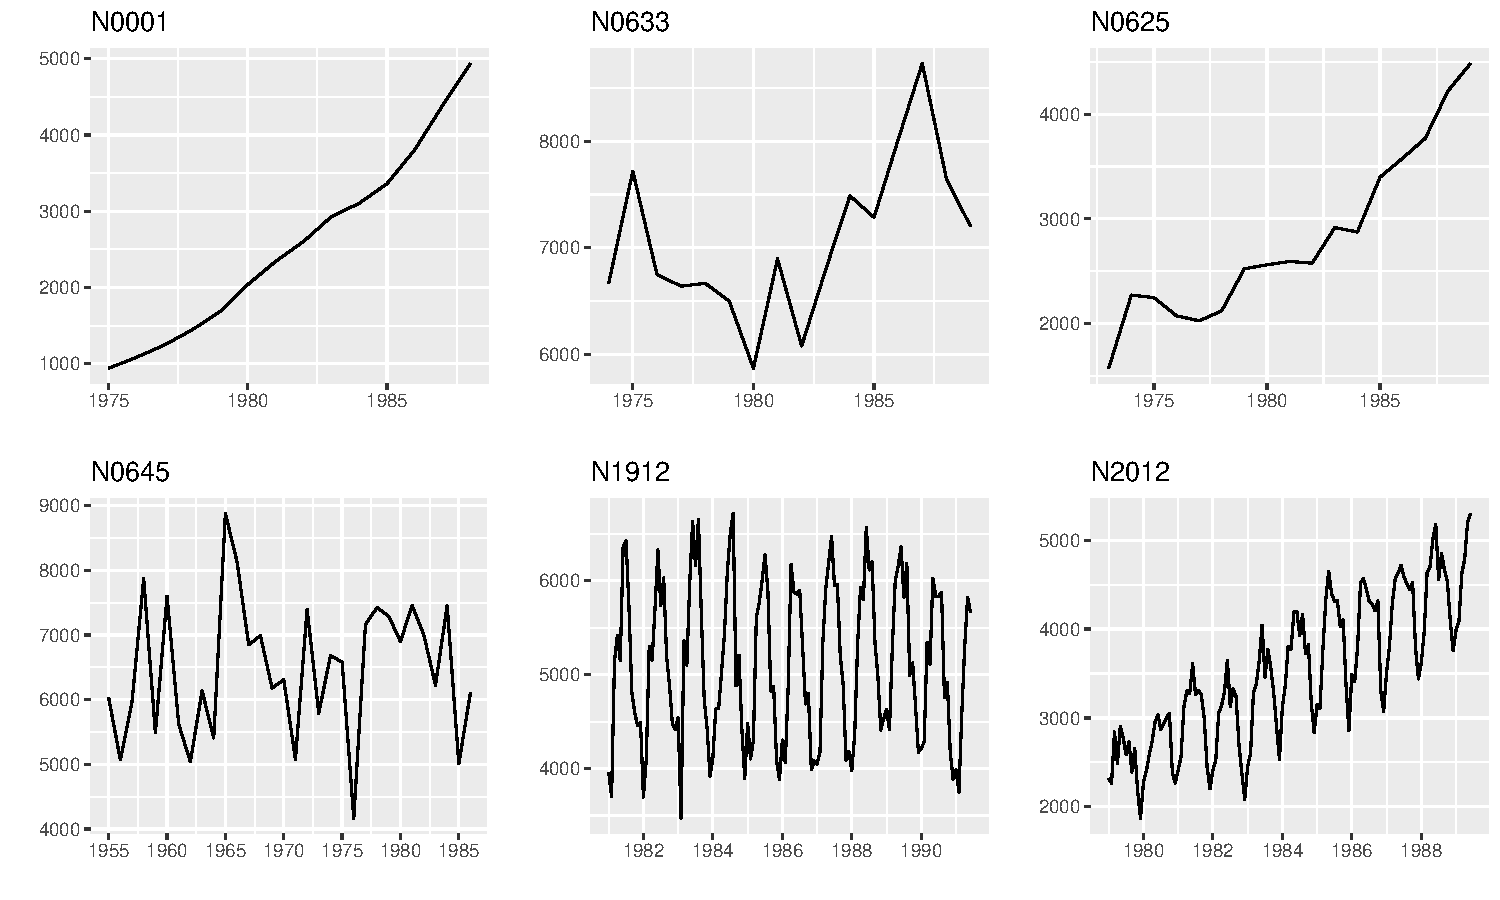
\includegraphics[width=\textwidth]{figure/fig1-1} 

}

\caption{Time-domain representation of time series}\label{fig:fig1}
\end{figure}

\begin{figure}

{\centering 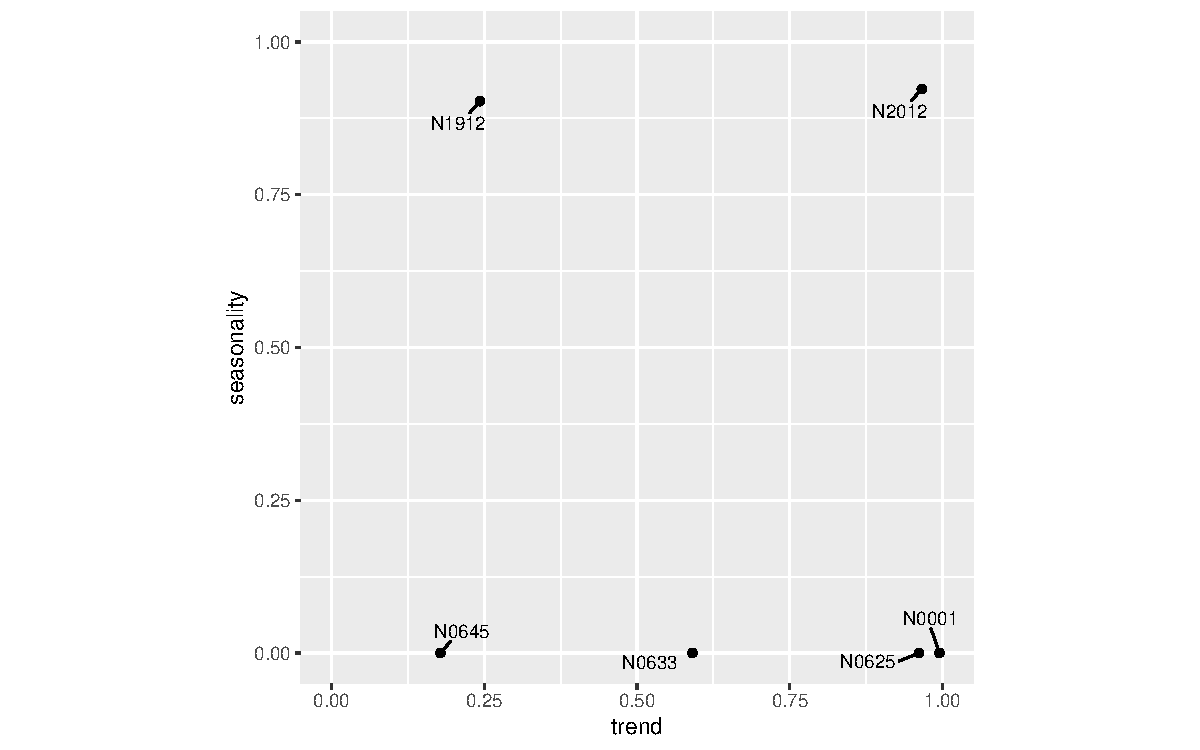
\includegraphics[width=0.7\linewidth]{figure/fig2-1} 

}

\caption{Feature-based representation of time series}\label{fig:fig2}
\end{figure}

The choice of the most appropriate set of features depends on both the nature of the time series being analysed, and the purpose of the analysis. In \autoref{Mcomp}, we study the time series from the M1 and M3 competitions \autocites{makridakis1982accuracy}{makridakis2000m3}, and we select features for the purpose of forecast-model selection. The M1 and M3 competitions involve time series of differing length, scale and other properties. We include length as one of our features, but the remaining features are independent of scale and asymptotically independent of the length of the time series (i.e., they are ergodic). As our main focus is forecasting, we select features which have discriminatory power in selecting a good model for forecasting.

\hypertarget{what-makes-features-useful-for-forecast-model-selection}{%
\subsection{What makes features useful for forecast-model selection?}\label{what-makes-features-useful-for-forecast-model-selection}}

\textcite{reid1972comparison} points out that the performance of forecasting methods changes according to the nature of the data. Exploring the reasons for these variations may be useful in selecting the most appropriate model. In response to the results of the M3 competition \autocite{makridakis2000m3}, similar ideas have been put forward by others. \textcite{hyndman2001s}, \textcite{lawrence2001s} and \textcite{armstrong2001s} argue that the characteristics of a time series may provide useful insights into which methods are most appropriate for forecasting.

Many time series forecasting techniques have been developed to capture specific characteristics of time series that are common in a particular discipline. For example, GARCH models were introduced to account for time-varying volatility in financial time series, and ETS models were introduced to handle the trend and seasonal patterns which are typical in quarterly and monthly sales data. An appropriate set of features should reveal the characteristics of the time series that are useful in determining the best forecasting method.

Several researchers have introduced rules for forecasting based on features \autocites{collopy1992rule}{adya2001automatic}{wang2009rule}. Most recently \textcite{kang2017visualising} applied principal component analysis to project a large collection of time series into a two dimensional feature space in order to visualize what makes a particular forecasting method perform well or not. The features they considered were spectral entropy, first-order auto-correlation coefficient, strength of trend, strength of seasonality, seasonal period and the optimal Box-Cox transformation parameter. They also proposed a method for generating new time series based on specified features.

\hypertarget{meta-learning-for-algorithm-selection}{%
\subsection{Meta-learning for algorithm selection}\label{meta-learning-for-algorithm-selection}}

John Rice was an early and strong proponent of the idea of meta-learning, which he called the algorithm selection problem (ASP) \autocite{rice1976}. The term \emph{meta-learning} started to appear with the emergence of the machine-learning literature. Rice's framework for algorithm selection is shown in \autoref{fig:rice} and comprises four main components. The problem space, \(P\), represents the data sets used in the study. The feature space, \(F\), is the range of measures that characterize the problem space \(P\). The algorithm space, \(A\), is a list of suitable candidate algorithms which can be used to find solutions to the problems in \(P\). The performance metric, \(Y\), is a measure of algorithm performance such as accuracy, speed, etc. A formal definition of the algorithm selection problem is given by \textcite{smith2009cross}, and repeated below.

\begin{quote}
\textbf{Algorithm selection problem}. For a given problem instance \(x \in P\), with features \(f(x) \in F\), find the selection mapping \(S(f(x))\) into algorithm space \(A\), such that the selected algorithm \(\alpha \in A\) maximizes the performance mapping \(y(\alpha(x)) \in Y\).
\end{quote}

\begin{figure}

{\centering 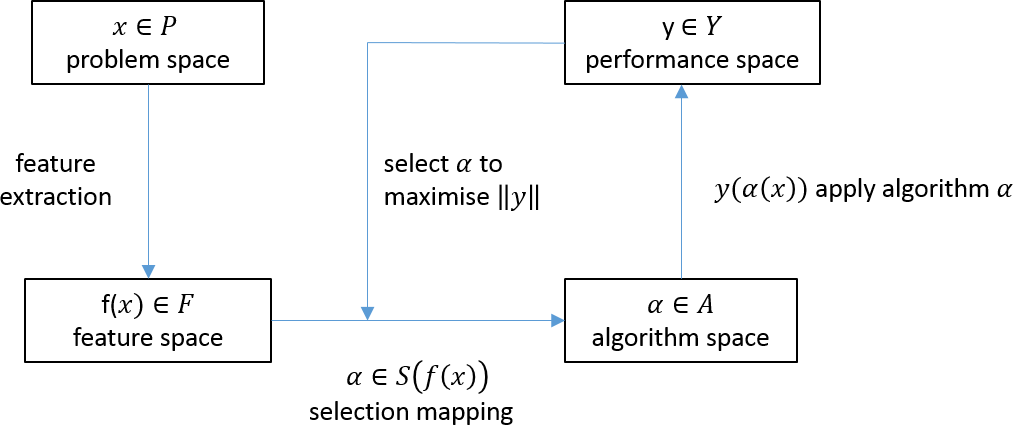
\includegraphics[width=0.8\linewidth]{images/RiceFramework} 

}

\caption{Rice's framework for the Algorithm Selection Problem.}\label{fig:rice}
\end{figure}

The main challenge in ASP is to identify the selection mapping \(S\) from the feature space to the algorithm space. Even though Rice's framework articulates a conceptually rich framework, it does not specify how to obtain \(S\). This gives rise to the meta-learning approach.

\hypertarget{forecast-model-selection-using-meta-learning}{%
\subsection{Forecast-model selection using meta-learning}\label{forecast-model-selection-using-meta-learning}}

Selecting models for forecasting can be framed according to Rice's ASP framework.

\begin{quote}
\textbf{Forecast-model selection problem}. For a given time series \(x \in P\), with features \(f(x) \in F\), find the selection mapping \(S(f(x))\) into the algorithm space \(A\), such that the selected algorithm \(\alpha \in A\) minimizes forecast accuracy error metric \(y(\alpha(x)) \in Y\) on the test set of the time series.
\end{quote}

Existing methods differ with respect to the way they define the problem space (\(A\)), the features (\(F\)), the forecasting accuracy measure (\(Y\)) and the selection mapping (\(S\)).

\textcite{collopy1992rule} introduced 99 rules based on 18 features of time series, in order to make forecasts for economic and demographic time series. This work was extended by \textcite{armstrong2001s} to reduce human intervention.

\textcite{shah1997model} used the following features to classify time series: the number of observations, the ratio of the number of turning points to the length of the series, the ratio of number of step changes, skewness, kurtosis, the coefficient of variation, autocorrelations at lags 1--4, and partial autocorrelations at lag 2--4. Casting Shah's work in Rice's framework, we can specify: \(P=203\) quarterly series from the M1 competition \autocite{makridakis1982accuracy}; \(A=3\) forecasting methods, namely simple exponential smoothing, Holt-Winters exponential smoothing with multiplicative seasonality, and a basic structural time series model; \(Y=\) mean squared error for a hold-out sample. \textcite{shah1997model} learned the mapping \(S\) using discriminant analysis.

\textcite{prudencio2004meta} was the first paper to use the term ``meta-learning'' in the context of time series model selection. They studied the applicability of meta-learning approaches for forecast-model selection based on two case studies. Again using the notation above, we can describe their first case study with: \(A\) contained only two forecasting methods, simple exponential smoothing and a time-delay neural network; \(Y=\) mean absolute error; \(F\) consisted of 14 features, namely length, autocorrelation coefficients, coefficient of variation, skewness, kurtosis, and a test of turning points to measure the randomness of the time series; \(S\) was learned using the C4.5 decision tree algorithm. For their second study, the algorithm space included a random walk, Holt's linear exponential smoothing and AR models; the problem space \(P\) contained the yearly series from the M3 competition \autocite{makridakis2000m3}; \(F\) included a subset of features from the first study; and \(Y\) was a ranking based on error. Beyond the task of forecast-model selection, they used the NOEMON approach to rank the algorithms \autocite{kalousis1999noemon}.

\textcite{lemke2010meta} studied the applicability of different meta-learning approaches for time series forecasting. Their algorithm space \(A\) contained ARIMA models, exponential smoothing models and a neural network model. In addition to statistical measures such as the standard deviation of the de-trended series, skewness, kurtosis, length, strength of trend, Durbin-Watson statistics of regression residuals, the number of turning points, step changes, a predictability measure, nonlinearity, the largest Lyapunov exponent, and auto-correlation and partial-autocorrelation coefficients, they also used frequency domain based features. The feed forward neural network, decision tree and support vector machine approaches were considered to learn the mapping \(S\).

\textcite{wang2009rule} used a meta-learning framework to provide recommendations as to which forecast method to use to generate forecasts. In order to evaluate forecast accuracy, they introduced a new measure \(Y =\) \emph{simple percentage better (SPB)}, which calculates the forecasting accuracy of a method against the forecasting accuracy error of random walk model. They used a feature set \(F\) comprising nine features: strength of trend, strength of seasonality, serial correlation, nonlinearity, skewness, kurtosis, self-similarity, chaos and periodicity. The algorithm space \(A\) included eight forecast-models, namely, exponential smoothing, ARIMA, neural networks and random walk model; while the mapping \(S\) was learned using the C4.5 algorithm for building decision trees. In addition, they used SOM clustering on the features of the time series in order to understand the nature of time series in a two-dimensional setting.

The set of features introduced by \textcite{wang2009rule} was later used by \textcite{widodomodel} to develop a meta-learning framework for forecast-model selection. The authors further reduced the dimensionality of time series by performing principal component analysis on the features.

More recently, \textcite{kuck2016meta} proposed a meta-learning framework based on neural networks for forecast-model selection. Here, \(P = 78\) time series from the NN3 competition were used to build the meta-learner. They introduced a new set of features based on forecasting errors. The average symmetric mean absolute percentage error was used to identify the best forecast-models for each series. They classify their forecast-models in the algorithm space \(A\), comprising single, seasonal, seasonal-trend and trend exponential smoothing. The mapping \(S\) was learned using a feed-forward neural network. Further, they evaluated the performance of different sets of features for forecast-model selection.

\printbibliography

\end{document}
